\chapter{Arquitectura de la solución}

En este capítulo vamos a describir la arquitectura que hemos diseñado para distribuir el bucle MAPE-K. Partimos de un sistema con una \textcolor{red}{división funcional ya definida}, por lo que será sencillo delimitar los componentes. El foco de este capítulo serán entonces los \textbf{conectores de \emph{software}}. Necesitamos establecer qué estrategias de comunicación utilizaremos para comunicar los componentes.

Comenzaremos dando una breve introducción a las arquitecturas de \emph{software} y los elementos que las componen. Después, describiremos la arquitectura de nuestra solución y el proceso que hemos seguido para llegar hasta ella.

\section{Arquitecturas de \emph{software}}

Según \cite{taylorSoftwareArchitectureFoundations2009}, la \textbf{arquitectura de un sistema \emph{software}} es el conjunto de todas las \textbf{decisiones principales de diseño} que se toman durante su ciclo de vida; aquellas que sientan las bases del sistema. Estas afectan a todos sus apartados: la funcionalidad que debe ofrecer, la tecnología para su implementación, cómo se desplegará, etc. En conjunto, definen una pauta que guía (y a la vez refleja) el diseño, la implementación, la operación y la evolución del sistema.

Todos los sistemas \emph{software} cuentan con una. La diferencia radica en si esta ha sido diseñada y descrita explícitamente o ha quedado implícita en su implementación. \cite{taylorSoftwareArchitectureFoundations2009} En el segundo caso es probable que, con el paso del tiempo, se ``erosione`` su arquitectura: se implementan funcionalidades sin respetar la estructura. También se olvida el por qué de ciertas decisiones. En general, se vuelve más difícil de mantener. Se convierte en una ''gran bola de barro''. \cite{footeBigBallMud1997}

Por tanto, es vital dedicar tiempo para definirla atendiendo a las necesidades de nuestro sistema. Una buena arquitectura es capaz dotar de estructura a nuestro sistema. \cite{martinCleanArchitectureCraftsman2018} Mientras se respete la arquitectura, y se mantenga actualizada, esta estructura. Una buena arquitectura nos ofrece una serie de ventajas, como facilitar su desarrollo, mayor extensibilidad.

\subsection{Componentes de una arquitectura}

Otra posible definición de arquitectura la encontramos en el estándar IEEE 42010-2011 \cite{ieeeStandard420102011Systems2011}: es "\emph{un conjunto de conceptos o propiedades fundamentales, personificados por sus elementos, sus relaciones, y los principios que guían su diseño y evolución}".

Podemos describirlas entonces usando tres conceptos: \cite{perryFoundationsStudySoftware1992}

    \begin{itemize}
        \item \textbf{Componentes} (o elementos): Son las piezas fundamentales que conforman el sistema. Representan las unidades de funcionalidad de la aplicación. Se utilizan para describir \textbf{\emph{qué}} partes componen el sistema. Por ejemplo: un módulo, un servicio web...

        \item \textbf{Forma}: El conjunto de propiedades y relaciones de un elemenento con otros o con el entorno de operación. Describe \textbf{\emph{cómo}} está organizado el sistema. Por ejemplo: un servicio A contacta con otro, B, usando una llamada HTTP.

        \item \textbf{Justificación}: Razonamiento o motivación de las decisiones que se han tomado. Responden al \textbf{\emph{por qué}} algo se hace de una manera determinada. Normalmente no pueden deducirse a partir de los elementos y la forma, por lo que es necesario describirlos explícitamente.

    \end{itemize}

\subsubsection{Elementos}

El primer tipo de elemento que debemos tratar son los componentes. Según \cite{taylorSoftwareArchitectureFoundations2009}, los \textbf{componentes} son ``elementos arquitectónicos que encapsulan un subconjunto de la funcionalidad y/o de los datos del sistema``.
Dependiendo de las características de nuestro sistema (y del nivel de abstracción que usemos) pueden tomar distintas formas: objetos, módulos dentro un mismo proceso, servicios distribuidos, etc.

\begin{wrapfigure}{r}{0.40\linewidth}
  \centering
  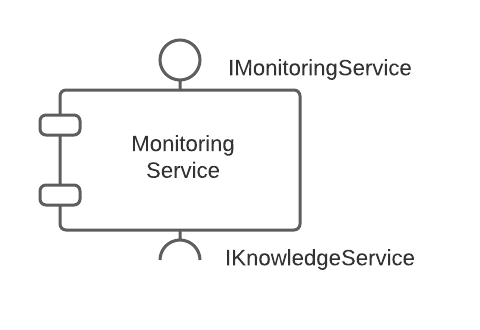
\includegraphics[scale=0.8]{03_arquitectura/images/componente-ejemplo}
  \caption{El servicio de monitorización representado como un componente. Ofrece una interfaz (\emph{IMonitoringService}) y depende de otra para funcionar (\emph{IKnowledgeService}).}
  \label{fig:componenteEjemplo}
\end{wrapfigure}

Los componentes exponen una \textbf{interfaz} que permite acceder a la funcionalidad o datos que encapsulan. A su vez, también declaran una serie de \textbf{dependencias} con interfaces de otros. Allí se incluyen todos los elementos que requieren para poder funcionar. En la figura \ref{fig:componenteEjemplo} tenemos un ejemplo. \emph{Monitoring Service} expone la interfaz \emph{IMonitoringService}. Para poder funcionar, depende de un componente que ofrezca \emph{IKnowledgeService}.

Por si solos, estos componentes independientes no aportan mucho valor. Más bien son la unidad básica de composición: podemos combinar varios de ellos para que trabajen conjuntamente y realicen tareas más complejas. Así, podemos \textbf{componer sistemas}. \cite{mehtaTaxonomySoftwareConnectors2000} La integración y la interacción entre ellos son aspectos clave que debemos abordar.

Para que dos o más componentes puedan interactuar, necesitamos definir un mecanismo de comunicación. Recurrimos entonces a los \textbf{conectores}. Se trata de elementos arquitectónicos que nos ayudan a definir y razonar sobre la comunicación entre componentes. En la figura \ref{fig:componentesYConectorEjemplo} mostramos una representación de la necesidad de comunicación entre dos componentes a través de un conector. No se ha especificado todavía ningún detalle sobre cómo se implementará. Así, podemos estudiar la arquitectura y elegir los mecanismos adecuados para cada interacción del sistema. \cite{taylorSoftwareArchitectureFoundations2009}.

%% TODO: Los conectores son application-independent. No dependen de la funcionalidad de la aplicación.
%% TODO: Hablar de la cardinalidad de los conectores.

\begin{figure}[h!]
  \centering
  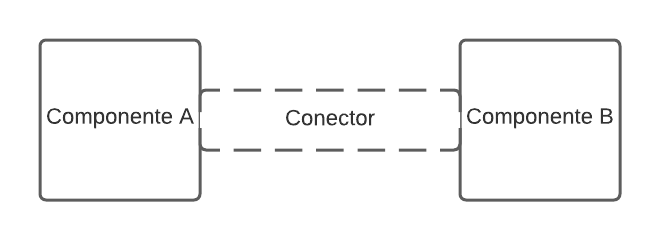
\includegraphics[scale=0.78]{03_arquitectura/images/conector}
  \caption{Ejemplo de comunicación de dos componentes a través de un conector.}
  \label{fig:componentesYConectorEjemplo}
\end{figure}

Internamente, los conectores están compuestos por uno o más \textbf{conductos} o canales. A través de estos se lleva a cabo la comunicación entre los componentes. Hay una gran variedad de conductos posibles: comunicación interproceso, a través de la red, etc. Clasificamos los conectores según la complejidad de los canales que utilizan \cite{mehtaTaxonomySoftwareConnectors2000}:

\pagebreak

\begin{itemize}
    \item \textbf{Conectores simples}: solo cuentan con un conducto, sin lógica asociada. Son conectores sencillos. Suelen estar ya implementados en los lenguajes de programación. Por ejemplo: una llamada a función en un programa o el sistema de entrada / salida de ficheros.

    \item \textbf{Conectores complejos}: cuentan con uno o más conductos. Se definen por composición a partir de múltiples conectores simples. Además, pueden contar con funcionalidad para manejar el flujo de datos y/o control. Suelen utilizarse importando \emph{frameworks} o librerias. Por ejemplo: un balanceador de carga que redirige peticiones a los nodos.
\end{itemize}

Por tanto, cuando hayamos decidido que dos componentes necesitan comunicarse, es momento de evaluar qué mecanismo de comunicación es más adecuado. Basándonos en nuestros requisitos, la arquitectura ya definida, y los mecanismos de despliegue que queremos usar, elegimos el conector apropiado. Podemos orientarnos con taxonomías como la de \cite{mehtaTaxonomySoftwareConnectors2000}.

\subsubsection{Forma}

\textcolor{red}{TODO:  - ¿Borrar?  Innecesario}

\subsubsection{Justificación}

\textcolor{red}{TODO:  - ¿Borrar?  Innecesario}

Una vez definidos los componentes, los conectores y las relaciones entre ellos, tendremos una representación del sistema. Pero se trata de una imagen incompleta. No cuenta con ciertos detalles del contexto que nos ayudan a entenderlo mejor. Un ejemplo podría ser qué alternativas se consideraron y por qué se descartaron en favor de la elegida. Tampoco contamos con detalles minuciosos que puedan guiar mejor la implementación.

Es decir, requerimos de un concepto adicional para describirlos en nuestra arquitectura: se trata de la \textbf{justificación}. \cite{perryFoundationsStudySoftware1992} Nos aporta detalles más precisos sobre el sistema que no se pueden representar como elementos o forma.

\subsection{Estilos arquitectónicos}

\textcolor{red}{TODO:  - ¿Borrar?  Innecesario}

\textcolor{red}{Podemos agrupar decisiones principales.}

\section{Arquitectura de la solución}

Como comentamos en el capítulo \ref{chap:introduccion}, el objetivo del trabajo es transformar un servicio monolítico en un sistema distribuido basado en microservicios. Se trata de un cambio arquitectónico importante. Queremos por tanto diseñar una estrategia ingenieril para llevar a a cabo la migración; teniendo en cuenta las particularidades del sistema.

El servicio en cuestión implementa un \textbf{bucle de control MAPE-K}\cite{ibmcorporationArchitecturalBlueprintAutonomic2006,fonsServiciosAdaptivereadyPara2021}, que ya describimos en la sección \ref{sub:bucles-mapek}.

En esta sección presentaremos nuestra propuesta arquitectónica para adaptar el bucle para entornos en la nube.

\textcolor{red}{Buscar libros de descomposición de monolitos en microservicios.}

\subsection{Distribución de los componentes}

Actualmente, el bucle está muy acoplado a los modelos de sus recursos manejados. Todo corre bajo el mismo proceso: el bucle, los monitores, sus reglas de adaptación y demás elementos específicos de la solución\dots Ese proceso solo podrá manejar aquellos sistemas cuyos módulos tenga cargados. En la figura \ref{fig:bucle-mapek2} presentamos otra vista de la arquitectura del bucle.

\begin{figure}[htb]
  \centering
  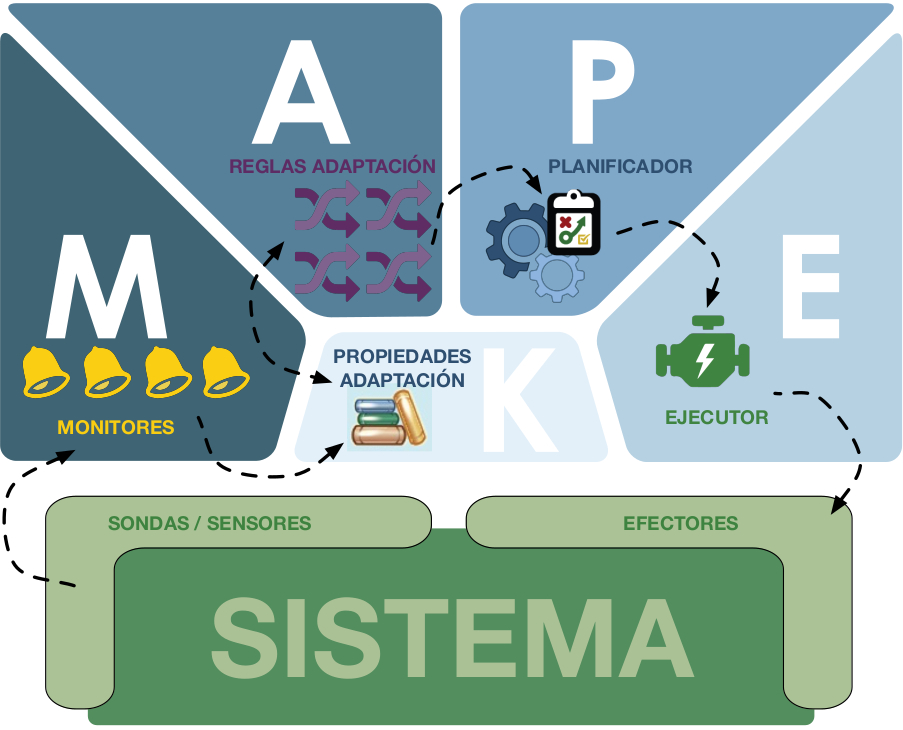
\includegraphics[scale=1.15]{01_introduccion/images/bucle-mape-k}
  \caption[Arquitectura de un Bucle MAPE-K. Podemos apreciar el flujo de información y de control a lo largo de las etapas del bucle.]{Arquitectura de un Bucle MAPE-K. Podemos apreciar el flujo de información y de control a lo largo de las etapas del bucle. Obtenida de \cite{fonsEspecificacionSistemasAutoadaptativos2021}}
  \label{fig:bucle-mapek2}
\end{figure}

Partimos entonces el objetivo de desacoplarlo. Así, podremos desplegarlo y usarlo de forma agnóstica al recurso manejado. La misma infraestructura podrá aprovecharse para manejar varios sistemas simultáneamente (\emph{multi-tennancy}). La idea es implementarlo a nivel de sistema\cite{mendoncaGeneralityVsReusability2018}, por lo que se desplegará al mismo con los microservicios del recurso manejado.

Como veremos a continuación, cada uno de sus componentes es candidato a convertirse en un microservicio individual.

Por la descripción de ambos componentes, vemos que existe una clara división de dominios y responsabilidades. Esto nos ayuda a determinar que ambos componentes pueden desplegarse por separado. \textcolor{red}{REFERENCIA 'Building Microservices' Sam Newman}

Por suerte, partimos de un sistema existente, con una arquitectura bien definida y documentada. Conocíamos el rol de cada uno de los componentes del servicio y sus requisitos. Asi que, el primer problema al que nos enfrentamos estaba relacionado con la distribución de los servicios. ¿Cómo definimos las fronteras entre cada uno de ellos? ¿Qué componentes debe abarcar cada microservicio?

La primera decisión que tomamos fue desacoplar el bucle de los sistemas. Buscábamos desarrollar microservicios agnósticos a la solución manejada. Por ello, vamos a identificar distintos \textbf{niveles de componentes} \textcolor{red}{Imagen que separa el bucle de la lógica de la solución.} Esto nos permitiría dar servicio a varios sistemas distintos con la misma infraestructura. Multi-tennancy.

Otra decisión que tomamos fue separar cada etapa del bucle en su propio servicio. Así podríamos independizarlas y escalarlas individualmente.

Una vez determinadas las fronteras entre los microservicios, hemos definido los componentes de nuestro sistema.

\begin{figure}[htb]
  \centering
  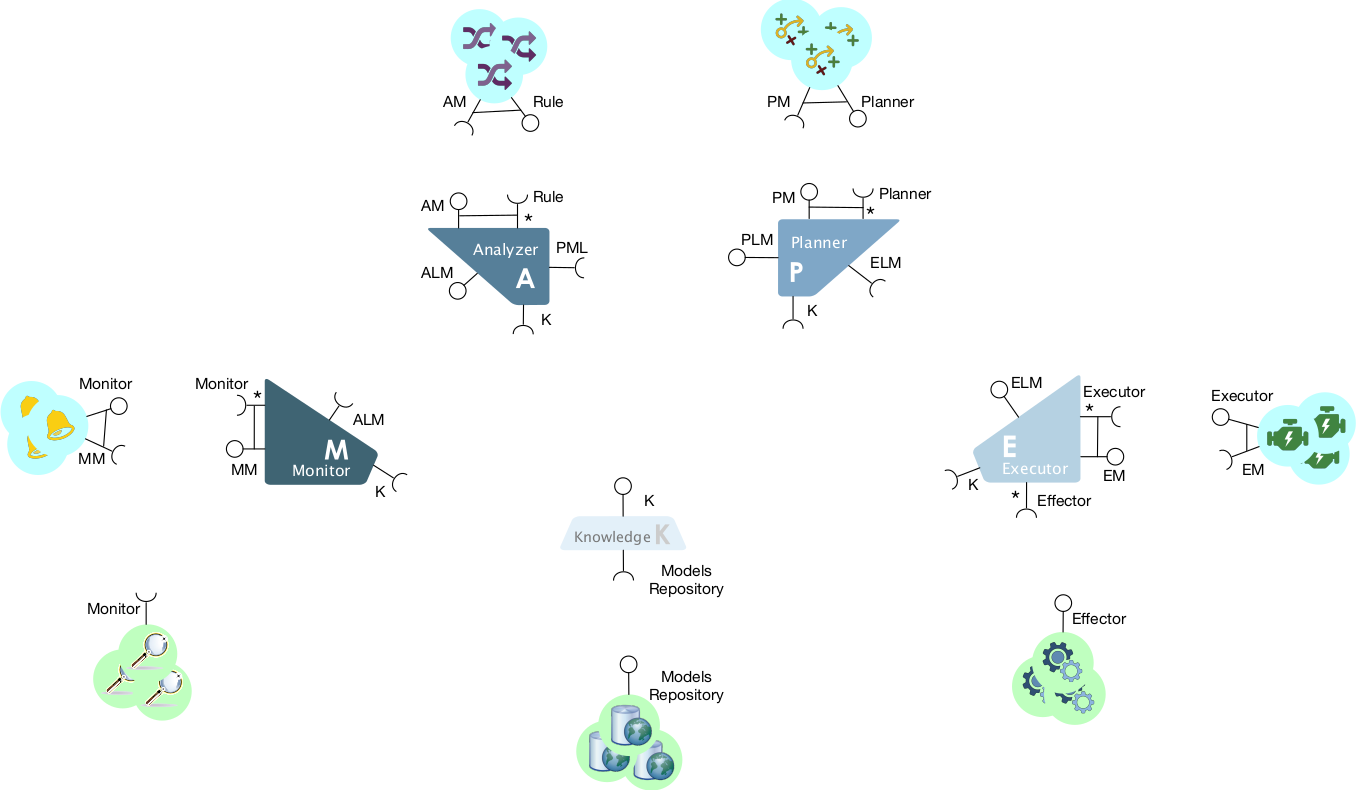
\includegraphics[scale=0.3]{03_arquitectura/images/mape-k-microservices}
  \caption{Diagrama con los componentes que forman nuestra arquitectura distribuida}
  \label{fig:mape-k-microservices}
\end{figure}

\textcolor{red}{Figura \ref{fig:mape-k-microservices}: Agrupar los servicios para poder aumentar zoom y hacerlo más legible. Añadir línea de divisón entre la capa del bucle y el dominio del recurso manejado.}

\subsection{Conectando los servicios}

El siguiente problema al que nos enfrentamos está relacionado con la comunicación: si dividimos estos componentes en microservicios, ¿cómo hacemos para que se comuniquen? Hay que tener en cuenta que estos pueden estar desplegados y replicados en distintas máquinas. No podemos asumir que están en el mismo \emph{host}.

Aprovechando la separación entre bucle de control y el dominio del recurso, investigamos posibles arquitecturas. Nos decantamos por \textbf{arquitecturas de servicios jerarquizados}. Queríamos explotar esta separación para mantener al bucle aislado del dominio de la solución. Dimos con el estilo arquitectónico C2 (\emph {components and connectors})\cite{taylorComponentMessagebasedArchitectural1996a, UCISoftwareArchitecture}, en el que nos hemos inspirado.

\subsubsection{Jerarquías de microservicios: Arquitectura C2 y arquitectura limpia}

Este estilo organiza sus componentes en jerarquías o capas: cada servicio se encuentra en un nivel determinado, según su nivel de abstracción. En las capas inferiores, se encuentran los servicios más externos, más ''acoplados'' al entorno. Por ejemplo, aquellos servicios que requieran de acceder al sistema de ficheros, estarían en esta capa. Por otro lado, en las capas superiores se encuentran los servicios en niveles de abstracción superior, que dependen lo mínimo del entorno.

En cuanto a la comunicación, un componente solo debe contactar con sus vecinos inmediatos (en una capa superior o inferior). Esto evita que el servicio pueda contactar con otras capas, limitando su alcance y su conocimiento del despliegue del sistema. Además, dentro del mismo nivel no pueden contactar entre ellos. Según la dirección de la comunicación, se emplean mecanismos distintos (figura \ref{fig:C2-arch-example}):

\begin{itemize}
  \item \textbf{Peticiones} (\emph{requests}): Se trata de solicitudes a un servicio para que ejecute una acción. Un componente se comunica directamente con un vecino en una capa superior. La petición viaja de ''fuera hacia dentro'' en cuanto al nivel de abstracción. Por ejemplo, una petición de un cliente a un servicio web podría estar bajo esta categoría.

  \item \textbf{Notificaciones}: Representan eventos ocurridos en el sistema. Un componente de más arriba en la jerarquía (más interno) envía un mensaje hacia abajo, sin especificar receptor. Todos los servicios por debajo lo recibirán, y decidirán si tratarlo o no. Esto evita que nuestro servicio se acople a aquellos que están por debajo (son más concretos). Un ejemplo sería notificar al resto de servicios sobre la creación de un nuevo usuario.
\end{itemize}

\begin{figure}[htb]
  \centering
  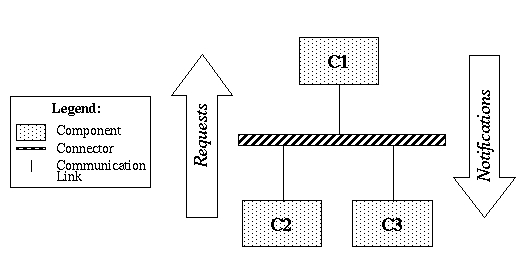
\includegraphics[scale=0.45]{03_arquitectura/images/c2SampleArch}
  \caption[Ejemplo del estilo arquitectónico C2 (\emph{Components and Connectors})]{Ejemplo del estilo arquitectónico C2 (\emph{Components and Connectors}). \cite{UCISoftwareArchitecture}}
  \label{fig:C2-arch-example}
\end{figure}

Basándonos en este estilo, definimos las capas de nuestro sistema. Esto nos permitió dividir los microservicios en niveles y elegir los conectores más adecuados para cada tipo de comunicación.

Distinguimos cuatro niveles distintos, de menor nivel de abstracción a mayor:

\begin{itemize}
  \item \textbf{Nivel del recurso manejado}: En este nivel se encuentran las sondas y efectores. Son los elementos que tienen más contacto con el recurso manejado. Hacen de intermediarios entre este y el resto del bucle, para reducir su acoplamiento.

  \item \textbf{\textcolor{red}{Nivel de específico solución}}: En esta capa se encuentran componentes del bucle específicos para el dominio del recurso manejado. Monitores específicos, reglas de adaptación... No los incluimos en el mismo nivel que las sondas y efectores porque necesitamos comunicar con ellos. Además que guardan más relación con el bucle que con el recurso manejado.

  \item \textbf{Nivel del bucle}: Aquí se encuentran los servicios de las etapas del bucle: servicio de monitorización, análisis, planificación y ejecución. Esta capa debe ser agnóstica al dominio de los recursos manejados. Además, actúa como intermediario entre los servicios de la solución y el conocimiento. Limitan cómo acceder a él.

  \item \textbf{Conocimiento}: Es la capa más interna y la base de la arquitectura. No depende de ningún otro componente, por lo que tiene el nivel de abstracción más alto. Todos los componentes del nivel del bucle dependen de ella para funcionar.

\end{itemize}

Habiendo definido esta jerarquía, vimos ciertas similitudes con arquitecturas \emph{domain driven}, como \emph{Clean Architecture}. \cite{martinChapter22Clean2018} En ella, el sistema se organiza en base a una \textbf{regla de dependencia}: \emph{''la dependencia entre los componentes solo puede apuntar hacia dentro, hacia políticas de alto nivel''}. Es decir, la arquitectura se organiza en capas concéntricas. En el centro se encuentra el dominio, con el mayor nivel de abstracción. Este no tiene dependencias con ninguna capa exterior. Por otro lado, cada capa más externa tiene dependencias sólo con la capa a la que envuelve. Sólo puede comunicarse con componentes dentro de esta.

Basándonos en la descripción anterior, nuestra capa central será la del conocimiento. A partir de ahí, cada nivel superior dependería de aquel al que ''envuelve'': el bucle al conocimiento, la solución al bucle...Por tanto, para que nuestra arquitectura sea más comprensible, optamos por representarla los diagramas de \emph{Clean Architecture} para representarlo. En la figura \ref{fig:clean-mapek-architecture} mostramos el resultado:

\begin{figure}[htb]
  \centering
  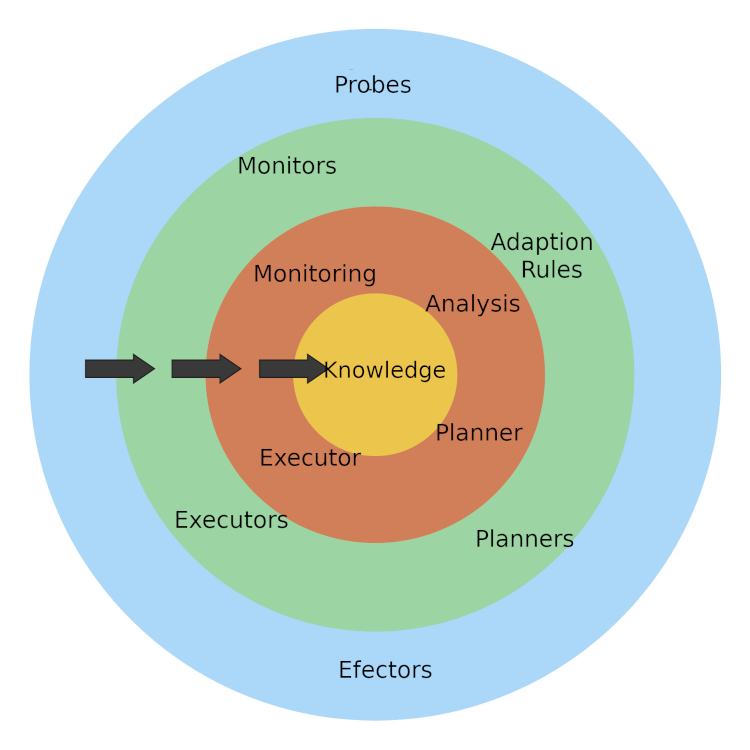
\includegraphics[scale=0.45]{03_arquitectura/images/clean-arch-2-MAPEK-style-small}
  \caption[Representación de nuestra propuesta arquitectónica. Inspirado en Arquitectura Limpia (\emph{Clean Architecture}). Las flechas negras representan las peticiones, y las moradas, las notificaciones.]{Representación de nuestra propuesta arquitectónica. Inspirado en Arquitectura Limpia (\emph{Clean Architecture}). Las flechas negras representan las peticiones, y las moradas, las notificaciones. \footnotemark }
  \label{fig:clean-mapek-architecture}
\end{figure}

\footnotetext{Imagen original de arquitectura limpia obtenida de: \url{https://threedots.tech/post/ddd-cqrs-clean-architecture-combined/}}

\subsubsection{Definiendo los mecanismos de comunicación}

Como comentamos antes, vamos a inspirarnos en los mecanismos de comunicación descritos por C2: las peticiones y notificaciones. Pero estos no cubren todas nuestras necesidades. Hay dos casos que no están contemplados: la comunicación del módulo de análisis con el planificador, y la del planificador con el ejecutor. Ambos módulos se encuentran en la misma capa. Y, como dependen del conocimiento, no podemos moverlos a una superior para utilizar notificaciones.

\textcolor{red}{Las notificaciones no nos sirven, ya que la comunicación es entre dos módulos específicos. Aunque nos interesa el desacoplamiento entre módulos que ofrecen. Las peticiones tampoco casan del todo, ya que requerimos desacoplar los módulos. Deberían mantener su independencia en el mayor grado posible.} Por ello, requerimos de un tercer patrón de comunicación. Una combinación de ambos: las peticiones asíncronas.

Los tres patrones de comunicaciones que usaremos entonces son:

\begin{itemize}
  \item \textbf{Peticiones síncronas}: Comunicaciones síncronas dirigidas a un servicio determinado. Solo permitidas entre servicios de una capa más externa a un servicio en la capa interior adyacente.

  \item \textbf{Peticiones asíncronas}: Comunicaciones asíncronas dirigidas a un servicio determinado. Solo están permitidas entre elementos del mismo nivel. Se trata de peticiones de trabajo de las cuales no requerimos una respuesta. Se envían y el destinatario lo procesará cuando pueda.

  \item \textbf{Notificaciones}: Comunicaciones asíncronas no dirigidas. El servicio publica un evento que potencialmente recibirán todos los servicios en la capa exterior adyacente. Tampoco esperamos ninguna respuesta.
\end{itemize}

\subsubsection{Conectores}

Una vez determinadas las necesidades de comunicación de nuestra arquitectura, debemos buscar los conectores adecuados. Seguimos la estrategia descrita en \cite{taylorSoftwareArchitectureFoundations2009} y consultamos patrones de comunicación en sistemas distribuidos descritos en \cite{newmanBuildingMicroservicesDesigning2021}.

Comenzamos investigando las peticiones síncronas. Tomemos por ejemplo la comunicación entre el servicio de monitorización (\emph{monitoring service}) y el servicio de conocimiento (\emph{knowledge service}). Recordemos que el servicio de conocimiento almacena todas las propiedades de adaptación. El resto de servicios necesitan consultarlas y actualizarlas durante su funcionamiento. En la figura \ref{fig:monitor-knowledge-initial} representamos inicialmente ambos componentes y un conector, sin especificar de qué tipo será.

% TODO: Cambiar por imagen de componentes, que ofrezcan y requieran interfaces.
\begin{figure}[htb]
  \centering
  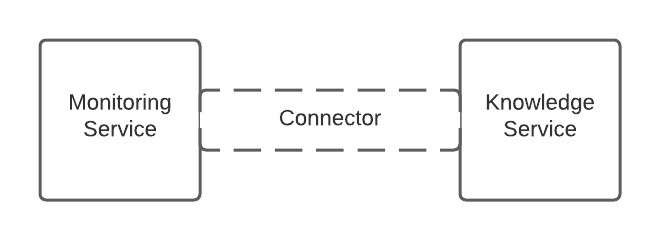
\includegraphics{03_arquitectura/images/Monitor-Knowledge-Initial-Connector}
  \caption{Boceto inicial: queremos conectar el servicio de monitorización con la base de conocimiento para poder leer propiedades de adaptación.}
  \label{fig:monitor-knowledge-initial}
\end{figure}

El siguiente paso es identificar qué interacciones debe existir entre ambos componentes. En este caso, el servicio de monitorización debe contactar con el servicio de conocimiento para leer y actualizar el valor de las propiedades. Por tanto, existen operaciones de lectura y escritura de los datos.

Ahora, debemos identificar qué \textbf{tipos de conector} serían adecuados para nuestros componentes. Sabiendo que hemos optado por una arquitectura distribuida, la elección se simplifica: los servicios pueden estar desplegados en máquinas distintas, por tanto el paso de mensajes será a través de la red.

Sabiendo esto, en lugar de recurrir a la taxonomía que lista \cite{mehtaTaxonomySoftwareConnectors2000}, optamos por consultar las estrategias de comunicación habituales para sistemas distribuidos descritas en \cite{newmanBuildingMicroservicesDesigning2021}. Se trata de cuatro mecanismos distintos: Invocación a métodos remotos (\emph{Remote Procedure Call}), APIs REST, consultas con GraphQL o \emph{brokers} de mensajería. Tuvimos que evaluarlos mediante un análisis de \emph{trade-offs} para determinar las ventajas y desventajas de cada uno.

\begin{itemize}
  \item \textbf{Invocación de métodos remotos} o (\emph{\textbf{Remote Procedure Call}}): Esta aproximación se basa en el estilo cliente-servidor. En ella, un servidor expone una serie de funciones que el cliente puede invocar mediante peticiones a través de la red. Estas peticiones incluyen el nombre de la función a ejecutar y sus parámetros. Al finalizar la ejecución, el servidor es capaz de devolver su resultado, si lo hubiera. Existen varios protocolos que implementan este mecanismo como gRPC o SOAP.

  Una evolución de RPC suele emplearse en la programación orientada a objetos: el paradigma de objetos distribuidos. \cite{tanenbaumChapter10Distributed2007} En este caso, el programa cliente interactúa con objetos que se encuentran en servidores remotos. Esta interacción se realiza a través de objetos que actúan como \emph{proxies}, abstrayendo de la llamada al servidor.

  Los \emph{proxies} ofrecen una interfaz para que el cliente invoque sus métodos localmente. Internamente, estos métodos realizan una llamada al servicio remoto donde se encuentra el objeto realmente. El servidor remoto procesa la petición y nos devolverá un resultado. Así, abstraen al cliente de todo este proceso de comunicación. En la figura \ref{fig:rpc-distributedobjects} tenemos un esquema de este mecanismo.

  \begin{figure}[htb]
    \centering
    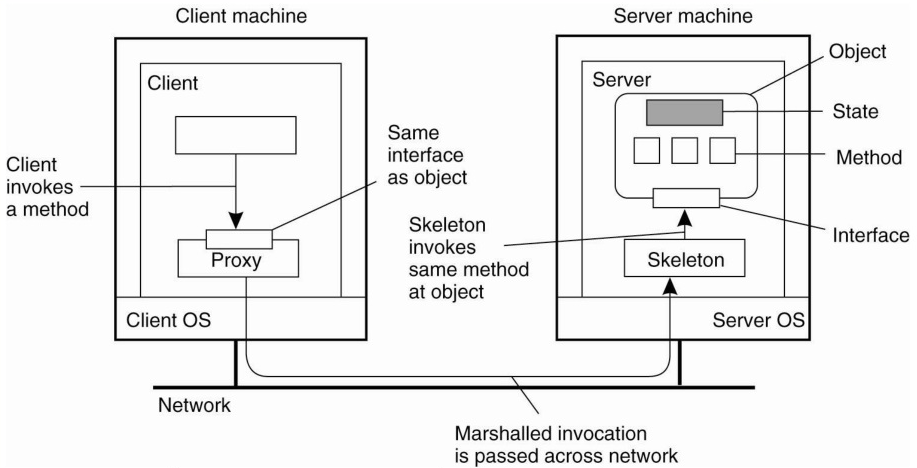
\includegraphics[scale=1.5]{03_arquitectura/images/rpc-distributedobjects}
    \caption[Funcionamiento del sistema de objetos distribuidos]{Funcionamiento del sistema de objetos distribuidos. \cite{tanenbaumChapter10Distributed2007}}
    \label{fig:rpc-distributedobjects}
  \end{figure}

  \begin{itemize}
    \item \textbf{Ventajas}:
    \begin{itemize}
      \item Permite la distribución del procesamiento del sistema.

      \item Abstrae al cliente de esta interacción con un servidor remoto. Para el cliente es prácticamente indistinguible de un objeto local.

      \item Los \emph{proxies} o (\emph{stubs} en la terminología de RPC) suelen generarse a partir de un contrato que define qué operaciones ofrecen estos objetos. Por ejemplo: SOAP con WDSL, gRPC; o en el caso de objetos distribuidos, Java RMI.
    \end{itemize}

    \item \textbf{Desventajas}:
    \begin{itemize}
      \item No se puede abstraer completamente al cliente de las llamadas a través de la red. Pueden darse errores que no ocurrirían durante una invocación de un método sobre un objeto local. Por ejemplo, que el servidor no esté disponible. \cite{jausovecFallaciesDistributedSystems2020}

      \item Dificulta la integración. Cada servicio ofrece sus propias funciones distintas.

      \item Si adoptamos sistemas como Java RMI, nuestro sistema se acopla a esa tecnología concreta. \cite{newmanBuildingMicroservicesDesigning2021}. Nos resta flexibilidad en cuanto a qué otras tecnologías podemos utilizar en nuestra arquitectura.

      \item El cliente debe actualizarse y recompilarse con cada cambio en el esquema del servidor. Esto puede ser problemático para casos donde tenemos que desplegar una actualización para que nuestros clientes puedan continuar utilizando la aplicación.
    \end{itemize}
  \end{itemize}

  \item \textbf{\emph{Representational State Transfer} (REST)}: Se basa también en el estilo arquitectónico cliente-servidor, pero con ciertas restricciones adicionales. \cite{taylorSoftwareArchitectureFoundations2009} Su concepto principal son los \textbf{recursos}: cualquier elemento del cual la API puede ofrecernos información y que pueda tener asociado un identificador único (una URI). \cite{richardsonRESTfulWebServices2007} Por ejemplo, podrían ser las entidades del dominio que gestiona nuestro servicio: Usuarios, Temperaturas\dots

  Las acciones que podemos ejecutar sobre los recursos (leer, crear, actualizar, \dots) las define el protocolo de comunicación sobre el que se implemente. Gracias a esto, la API que pueden ofrecer los servicios REST es común. Solo cambia el ``esquema de los datos``, los tipos de recursos que ofrecen. Esto facilita enormemente la integración con otros servicios. \cite{nallyRESTVsRPC2018} La implementación más común de REST es sobre el protocolo HTTP.

  \begin{itemize}
    \item \textbf{Ventajas}:

    \begin{itemize}
      \item \textbf{\emph{Stateless}}: El servidor no mantiene el estado de la sesión. Esto permite que cada petición sea independiente de las demás.

      \item \textbf{Escalable}: Como las sesiones deben ser \emph{stateless}, podremos replicar nuestro servicio y que distintas instancias puedan atender las peticiones que surjan durante la sesión.

      \item \textbf{API Sencilla}: Solo hay que implementar unos pocos métodos estándar para interactuar con la API.

      \item \textbf{Comunicación síncrona}: Es el mecanismo ideal para comunicaciones síncronas, donde el cliente requiere la respuesta del servicio para poder continuar con su procesamiento. También podemos dar soporte a para comunicaciones \emph{fire and forget}, donde el cliente envía un mensaje y no espera ninguna respuesta a su petición.

      \item \textbf{Interoperabilidad}: Ampliamente utilizado en servicios de Internet. Es ideal para que clientes externos contacten con nuestro sistema mediante peticiones síncronas. \cite{newmanBuildingMicroservicesDesigning2021}

      \item \textbf{Generación de clientes}: Para facilitar la comunicación con APIs REST, podemos generar librerias cliente utilizando el estándar OpenAPI. Lo explicaremos con maś detalle en la sección \ref{chap:OpenAPI}.
    \end{itemize}

    \item \textbf{Desventajas}:

    \begin{itemize}
      \item \textbf{Rendimiento}: El rendimiento es peor comparado con mecanismos RPC. El tamaño de un mensaje HTTP serializado en XML o JSON es mayor que si estuviera en un formato binario.

      \item \textbf{API Sencilla}: También es una desventaja. Hay operaciones complejas que es difícil representar con los métodos ofrecidos por el protocolo de comunicación. Pueden requerir más tiempo de diseño, o incluso ser implementados siguiendo RPC.
    \end{itemize}
  \end{itemize}

  \item \textbf{GraphQL}\footnote{Página oficial: \url{https://graphql.org/}} \textcolor{red}{AMPLIAR}: Se trata de un protocolo para que un cliente pueda hacer consultas personalizadas sobre los datos de un servidor. No necesitan que haya sido implementado con lógica asociada. De esta forma, se puede reducir la cantidad de peticiones a través de la red que se necesita ejecutar para obtener la misma información.

  \begin{itemize}
    \item \textbf{Ventajas}:

    \begin{itemize}
      \item \textbf{Ideal para móviles}: Gracias a que reduce la cantidad de llamadas, es ideal para entornos donde queremos optimizar el uso de datos.

      \item \textbf{Rendimiento}: Ofrece un mayor rendimiento comparado con otras alternativas que no ofrezcan un endpoint ya implementado. Y debamos obtener la misma información por composición, haciendo varias llamadas.
    \end{itemize}

    \item \textbf{Desventajas}:

    \begin{itemize}
      \item \textbf{Exponemos datos a la red}:

      \item \textbf{Problemas de rendimiento}: El cliente puede hacer consultas muy pesadas que penalicen el rendimiento de la base de datos sobre la que opera nuestro servicio.
    \end{itemize}
  \end{itemize}

  \item \textbf{\emph{Brokers} de mensajería}: Es un mecanismo de \textbf{comunicación asíncrona} muy popular. Sobre todo en arquitecturas basadas en eventos. Contamos con un servicio que actúa como intermediario, el \emph{broker}. Este gestiona la comunicación entre los servicios del sistema. \cite{newmanBuildingMicroservicesDesigning2021} Hay varias estrategias de comunicación posibles: punto a punto, \emph{publish-suscribe}, híbrida\dots

  Tomemos por ejemplo \emph{publish-suscribe}: es una estrategia para implementar comunicación \emph{multicast}. Se basa en el uso de \textbf{temas} o \textbf{\emph{topics}}, categorías de mensajes que pueden resultar de interés. Un servicio (el productor) envía un mensaje al \emph{broker}, indicando que pertenece a un tema determinado. El \emph{broker} recibe el mensaje y se encarga de reenviarlo a todos los servicios subscritos a este tema en cuanto sea posible. \cite{rabbitmqPublishSubscribeDocumentation} En la figura \ref{fig:publish-subscribe} tenemos un ejemplo de esta estrategia.

  \begin{figure}[htb]
    \centering
    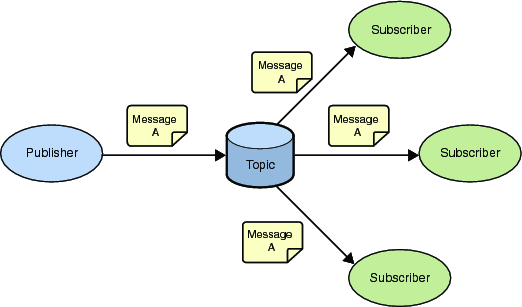
\includegraphics[scale=0.5]{03_arquitectura/images/publish_subscribe}
    \caption[Estrategia \emph{publish/suscribe}: el \emph{broker} actúa como intermediario en la comunicación \emph{multicast}.]{Estrategia \emph{publish/suscribe}: el \emph{broker} actúa como intermediario en la comunicación \emph{multicast}. Imagen obtenida de \footnotemark}
    \label{fig:publish-subscribe}
  \end{figure}

  \footnotetext{Java Messaging Service: \url{https://docs.oracle.com/cd/E19509-01/820-5892/ref_jms/index.html}}

  La mayor ventaja de este estilo de comunicación es el \textbf{desacoplamiento} entre los servicios. \cite{korabUnderstandingMessageBrokers2017}
  Ninguno de ellos necesita conocer detalles sobre cómo están desplegado los otros: su dirección, el número de instancias, si están activos en este momento, etc. Solo necesitan conocer la dirección del \emph{broker} para enviar o recibir mensajes.

  \begin{itemize}
    \item \textbf{Ventajas}:

    \begin{itemize}
      \item \textbf{Comunicación asíncrona}: El servicio no necesita quedarse a la espera de una respuesta del servidor. Puede procesar otras operaciones hasta que se le notifique del resultado, si lo hubiera.

      \item \textbf{Desacoplamiento de los servicios}: Ni los productores ni los consumidores necesitan conocer el origen o destino de sus mensajes.

      \item \textbf{Envío garantizado de mensajes}: El \emph{broker} garantiza que el mensaje será entregado \emph{al menos} una vez.

    \end{itemize}

    \item \textbf{Desventajas}:

    \begin{itemize}
      \item \textbf{Requisitos de infraestructura}: Utilizar un \emph{broker} de mensajería implica tener ciertas consideraciones a la hora de diseñar nuestro plan de despliegue. Estos sistemas requieren de replicación para alcanzar la alta disponibilidad necesaria para que sea fiable. \cite{newmanBuildingMicroservicesDesigning2021} Por tanto, aumenta la complejidad de operar el sistema.

      \item \textbf{Envío garantizado de mensajes}: Para poder garantizar el envío de un mensaje, el \emph{broker} puede recurrir a reenviarlo. Debemos diseñar nuestros sistemas de forma que estos mensajes duplicados, si ya han sido procesados, deben ser descartados.
    \end{itemize}
  \end{itemize}
\end{itemize}

De estas cuatro opciones, podemos descartar inmediatamente la opción de GraphQL. Se trata de un conector más orientado a las consultas de datos. En nuestro caso, necesitamos ejecutar también escrituras de los valores de las propiedades. Siguiendo también este razonamiento nos llevó a descartar el \emph{broker} de mensajería. Para obtener propiedades del conocimiento, resultaba más sencillo de implementar mediante comunicación síncrona.

Finalmente, hay que tener en cuenta que una de nuestras prioridades es la \textbf{interoperabilidad}: es una API expuesta ''hacia fuera'', hacia una capa más externa; prima por tanto la compatibilidad con cualquier tipo de cliente. Descartamos entonces RPC, dado que nos acoplaría a una tecnología concreta y a APIs no estándares.

Terminamos por tanto decantándonos por implementar la comunicación utilizando un conector REST sobre HTTP. Implementamos ambas funciones mediante \emph{endpoints} HTTP. Su especificación se detalla a continuación en las tablas \ref{tab:especificacion-get-property} y \ref{tab:especificacion-put-property}.

\newsavebox\getpropertyrequestbox
\begin{lrbox}{\getpropertyrequestbox}
  \begin{minipage}[t]{1in}
    \begin{verbatim}
Request:
HTTP GET property/currentTemperature

Response: 200 Ok
{
  value: {
    "Value":16.79,
    "Unit": 1, // Celsius
    "ProbeId":"c02234d3-329c-4b4d-aee0-d220dc25276b",
    "DateTime":"2022-01-15T18:19:38.5231231Z"
  },
  lastModification: "2022-01-15T18:19:39.123213Z"
}
    \end{verbatim}
  \end{minipage}
\end{lrbox}

\begin{table}[htb]
  \centering

  \begin{tabular}{|m{3.4cm}|p{2.5cm}|p{1cm}|p{3cm}|}
      \hline

      \textbf{Operación HTTP} & GET & \textbf{Ruta} & property/\{\emph{propertyName}\} \\
      \hline

      \textbf{Descripción} & \multicolumn{3}{|l|}{Devuelve el valor de la propiedad, si existe.} \\
      \hline

      \textbf{Parámetros} & \emph{propertyName} & \multicolumn{2}{|m{0.55\linewidth}|}{El nombre de la propiedad que deseamos obtener. Se lee a partir de la ruta de la petición.}\\
      \hline

      \multirow{3}*{\textbf{Respuestas posibles}}
            & \textbf{Código 200 (Ok)} & \multicolumn{2}{|m{0.55\linewidth}|}{La propiedad se ha encontrado. Incluye un \emph{payload} con el siguiente esquema:

            \begin{itemize}
              \item \emph{Value}: Valor de la propiedad serializado en JSON.
              \item \emph{LastModification}: Fecha y hora de la última modificación de esta propiedad.
            \end{itemize}}\\

            \cline{2-4}

            & \textbf{Código 400 (Bad request)} & \multicolumn{2}{|m{0.55\linewidth}|}{La petición está mal formada, no es acuerdo al contrato.}\\

            \cline{2-4}

            & \textbf{Código 404 (Not found)} & \multicolumn{2}{|m{0.55\linewidth}|}{No se ha encontrado ninguna propiedad con el nombre proporcionado.}\\
      \hline

      \textbf{Ejemplo} & \multicolumn{3}{|b{0.7\linewidth}|}{Petición para obtener la propiedad \emph{currentTemperature}:
      \usebox\getpropertyrequestbox} \\

      \hline
  \end{tabular}

  \caption{Especificación de la operación para obtener una propiedad del servicio de conocimiento.}
  \label{tab:especificacion-get-property}
\end{table}

\newsavebox\putpropertyrequestbox
\begin{lrbox}{\putpropertyrequestbox}
  \begin{minipage}[t]{2in}
    \begin{verbatim}
Request:
HTTP PUT property/currentTemperature

{
  value: {
    "Value":16.79,
    "Unit": 1, // Celsius
    "ProbeId":"c02234d3-329c-4b4d-aee0-d220dc25276b",
    "DateTime":"2022-01-15T18:19:38.5231231Z"
  }
}

Response: 204 (No content)
        \end{verbatim}
  \end{minipage}
\end{lrbox}

\begin{table}[htb]
  \centering

  \begin{tabular}{|m{3.4cm}|m{2.5cm}|b{1cm}|b{3cm}|}
      \hline

      \textbf{Operación HTTP} & PUT & \textbf{Ruta} & property/\{\emph{propertyName}\} \\
      \hline

      \textbf{Descripción} & \multicolumn{3}{|b{0.7\linewidth}|}{ Actualiza (o crea, si no existe) el valor de la propiedad con el nombre dado.} \\
      \hline

      \multirow{2}*{\textbf{Parámetros}}
            & \emph{propertyName} & \multicolumn{2}{|b{0.55\linewidth}|}{El nombre de la propiedad que deseamos crear o actualizar. Se lee a partir de la ruta de la petición.}\\

            \cline{2-4}

            & \emph{SetPropertyDTO} & \multicolumn{2}{|b{0.55\linewidth}|}{ Un DTO que contiene el valor a asignar en la propiedad serializado en JSON. El DTO se encuentra en el cuerpo de la petición.} \\
      \hline

      \multirow{2}*{\textbf{Respuestas posibles}}
            & \textbf{Código 204 (No content)} & \multicolumn{2}{|b{0.55\linewidth}|}{La propiedad se ha creado o actualizado correctamente. No incluye \emph{payload} en el cuerpo de la respuesta.}\\

            \cline{2-4}

            & \textbf{Código 400 (Bad request)} & \multicolumn{2}{|b{0.55\linewidth}|}{La petición está mal formada, no es acuerdo al contrato.}\\
      \hline

      \textbf{Ejemplo} & \multicolumn{3}{|b{0.7\linewidth}|}{Petición para actualizar la propiedad \emph{currentTemperature} con una medición de un termómetro:
      \usebox\putpropertyrequestbox} \\

      \hline
  \end{tabular}

  \caption{Especificación de la operación para actualizar o crear una propiedad del servicio de conocimiento.}
  \label{tab:especificacion-put-property}
\end{table}

Una vez definida la interfaz que expondrá el servicio de conocimiento, nos queda definir cómo se contactará desde el servicio de monitorización. ¿Implementamos las llamadas manualmente con un cliente HTTP? Aunque no sería muy complicado, tendríamos que mantenerlo manualmente cuando evolucione el sistema. Optamos entonces por una alternativa: el estándar OpenAPI.

\subsection{Open API}
\label{chap:OpenAPI}

\begin{wrapfigure}{r}{0.3\linewidth}
  \vspace{5pt}
  
\includegraphics[scale=0.32]{03_arquitectura/images/openapi-logo}
  \centering
  \vspace{5pt}
\end{wrapfigure}

OpenAPI es un lenguaje estándar para describir APIs RESTful. Nos permite describir de forma estructurada las operaciones que ofrece un servicio HTTP, manteniéndose agnóstico a su implementación. Esta descripción ayuda tanto a humanos como a computadoras a descubrir y utilizar las funcionalidades de la API. La OpenAPI Initiative (OAI) dirige el proyecto bajo el manto de la \emph{Linux Foundation}.

Un documento OpenAPI habitual documenta el funcionamiento de la API y el conjunto de recursos que la componen. Describe las operaciones HTTP que podemos ejecutar sobre estos recursos, incluyendo las estructuras de datos que recibe o envía y los códigos de respuesta. Estos códigos indican al cliente el resultado de la ejecución de la operación. \cite{openapi_initiativeOpenAPISpecificationV3} Más adelante mostraremos un ejemplo, con el \textcolor{red}{fragmento} \ref{ls:openapi-get}.

La especificación puede escribirse manualmente o puede generarse a partir de una implementación existente. Así, podemos desarrollar nuestro servicio en un determinado lenguaje y obtener su descripción en OpenAPI. Podemos aprovecharla en varios ámbitos del desarrollo, gracias a la gran variedad de herramientas existentes: generación de documentación, generación de casos de prueba, identificar cambios incompatibles, etc. \cite{westerveldChapterOpenAPIAPI2021}

Uno de los casos de uso más interesantes es la generación de código a partir de la definición. Existen una serie de generadores\footnote{\url{https://github.com/OpenAPITools/openapi-generator}} capaces de generar clientes o servidores conformes a la especificación. Ofrecen soporte a una gran variedad de lenguajes: Java, C\#, JavaScript\dots En el caso de cliente, actúa como un proxy que nos abstrae de la lógica de comunicación con el servidor, similar a lo descrito en el apartado de RPC.

Para el desarrollo de este trabajo, nos interesaba especialmente debido a las diferencias tecnológicas existentes: el bucle MAPE-K original estaba desarrollado en Java, pero el prototipo se desarrolló con el lenguaje C\# junto con el framework ASP.NET Core. Se tomó esta decisión para reducir el tiempo de aprendizaje y centrar los esfuerzos en la definición de la arquitectura del sistema.

\textcolor{red}{Gracias a la generación de código, pudimos obtener la especificación de los servicios desarrollados en ASP.NET Core, y generar clientes o servidores en cualquier lenguaje soportado, Java incluido. El bucle MAPE-K original después podría ser refactorizado usando este código autogenerado.}

\subsubsection{Ejemplo de uso}

A continuación explicaremos brevemente cómo utilizamos OpenAPI para documentar nuestras APIs y generar la especificación estas. Para ello, continuaremos con el ejemplo del servicio de conocimiento que hemos descrito a lo largo de este capítulo. Vamos a centrarnos en la implementación de la operación para obtener una propiedad del conocimiento, que describimos en la tabla \ref{tab:especificacion-get-property}.

En el \textcolor{red}{fragmento} \ref{ls:csharp-get}, podemos observar que se trata de un método C\# llamado \emph{GetProperty}. Su implementación es sencilla: busca en un diccionario la propiedad cuyo nombre se le pasa por parámetro. En caso de encontrarla, devuelve su valor con un código 200 OK. En caso contrario, devuelve un código de error que describe qué ha ocurrido exactamente (llamada incorrecta o no se ha encontrado la propiedad).

Aparte de la implementación, podemos comprobar que el método se ha decorado con una serie de comentarios (líneas 1-8) y atributos (10-12). Esta documentación describe qué hace el método, sus entradas y posibles respuestas. OpenAPI es capaz de utilizar estos elementos opcionales para generar una especificación más completa. Por tanto, resulta muy recomendable utilizarlos.

\begin{lstlisting}[language={[Sharp]C},caption={Implementación del método GetProperty decorado para generar la especificación OpenAPI.},captionpos=b, label=ls:csharp-get]
/// <summary>
///    Gets a property given its name.
/// </summary>
/// <param name="propertyName"> The name of the property to find. </param>
/// <returns> An IActionResult with result of the query. </returns>
/// <response code="200"> The property was found. Returns the value of the property. </response>
/// <response code="404"> The property was not found. </response>
/// <response code="400"> There was an error with the provided arguments. </response>
[HttpGet("{propertyName}")]
[ProducesResponseType(typeof(PropertyDTO), StatusCodes.Status200OK)]
[ProducesResponseType(StatusCodes.Status404NotFound)]
[ProducesResponseType(StatusCodes.Status400BadRequest)]
public IActionResult GetProperty([FromRoute]string propertyName)
{
    if (string.IsNullOrEmpty(propertyName))
    {
        return BadRequest();
    }

    bool foundProperty = properties.TryGetValue(propertyName, out PropertyDTO property);

    if (!foundProperty)
    {
        return NotFound();
    }

    return Ok(property);
}
\end{lstlisting}

Haciendo uso de las librerías de OpenAPI, generamos la especificación a partir del servicio de conocimiento. En el \textcolor{red}{fragmento} \ref{ls:openapi-get}, podemos ver cómo se describe la operación en este estándar:

\begin{lstlisting}[language=python,caption={Especificación OpenAPI del método para obtener una propiedad del conocimiento (\lstinline{GetProperty}).},captionpos=b, label=ls:openapi-get]
"paths": {
  "/Property/{propertyName}": {
    "get": {
      "tags": [
        "Property"
      ],
      "summary": "Gets a property given its name.",
      "parameters": [
        {
          "name": "propertyName",
          "in": "path",
          "description": "The name of the property to find.",
          "required": true,
          "schema": {
            "type": "string"
          }
        }
      ],
      "responses": {
        "200": {
          "description": "The property was found. Returns the value of the property.",
          "content": {
            "application/json": {
              "schema": {
                "$ref": "#/components/schemas/PropertyDTO"
              }
            }
          }
        },
        "404": {
          "description": "The property was not found.",
        },
        "400": {
          "description": "There was an error with the provided arguments.",
        }
      }
    }
  }
\end{lstlisting}

Podemos apreciar que en la ruta (\emph{/Property/\{propertyName\}}) está disponible una operación de tipo \emph{get} y que acepta determinados parámetros y ofrece unas posibles respuestas. Aparece una referencia a otro esquema (línea 25), que representa la estructura de la respuesta en ese caso concreto. También aparecen los comentarios opcionales que indicamos en el \textcolor{red}{fragmento} \ref{ls:csharp-get}. Encontramos grandes similitudes con la especificación presentada en la tabla \ref{tab:especificacion-get-property}.

Los convenios de los generadores de código de OpenAPI pueden no ser de nuestro agrado. Por ejemplo, pueden resultar muy verbosos o puede resultar muy pesado trabajar con DTOs directamente. Por suerte, tenemos dos opciones para solventar esto: Modificar las plantillas de generación de código. Al ser de código abierto, podríamos modificar las existentes o crear nuestras propias plantillas con nuestros propios convenios.

Otra opción, más fácil de implementar, es desarrollar código por encima del API Client Generado. Es el caso del servicio de Análisis. Como trabajar con DTOs directamente se hacía muy pesado, optamos por implementar un `system configuration request` builder. Esto nos permitia configurar la petición de una forma más descriptiva para el usuario:

\begin{lstlisting}[language={[Sharp]C},caption={Implementación de la misma petición siguiendo el patrón \emph{builder}.},captionpos=b, label=ls:api-cliente-request-builder]
var changeRequests = new List<ServiceConfigurationDTO>
{
  new()
  {
    ServiceName = ClimatisationAirConditionerConstants.AppName,
    IsDeployed = true,
    ConfigurationProperties = new List<ConfigurationProperty>()
    {
      new()
      {
          Name = ClimatisationAirConditionerConstants.Configuration.Mode,
          Value = AirConditioningMode.Cooling.ToString(),
      },
    },
  },
};

var symptoms = new List<SymptomDTO> { new(SymptomName, "true") };

var systemConfigurationChangeRequest = new SystemConfigurationChangeRequestDTO()
{
  ServiceConfiguration = changeRequests,
  Symptoms = symptoms,
  Timestamp = DateTime.UtcNow,
};

await _systemApi.SystemRequestChangePostAsync(
  systemConfigurationChangeRequest,
  CancellationToken.None);
\end{lstlisting}


\begin{lstlisting}[language={[Sharp]C},caption={Implementación de la misma petición siguiendo el patrón \emph{builder}.},captionpos=b, label=ls:api-cliente-request-builder]
await _systemService.RequestChangeAsync(changeRequest =>
{
  changeRequest
    .ForSymptom(TemperatureGreaterThanHotThreshold)
    .WithService(ClimatisationAirConditionerConstants.AppName, service =>
    {
      service.MustBePresent()
        .WithParameter(
          ClimatisationAirConditionerConstants.Configuration.Mode,
          AirConditioningMode.Cooling.ToString());
    });
});
\end{lstlisting}

Finalmente, la arquitectura del conector que emplearemos para implementar las peticiones aparece en la figura \ref{fig:monitor-knowledge-connector-architecture}. La figura muestra como el servicio de monitorización contacta al de conocimiento para asignarle un valor a la propiedad \emph{Temp}.

El conector, delimitado por una línea discontinua roja, está compuesto por dos elementos: una API REST y un cliente. Los otros dos grupos de elementos representan los procesos de los servicios de monitorización y conocimiento. El servicio de monitorización se comunica a con la API través del API Client, que está en su proceso actuando como \emph{proxy}.

%%% TODO: Actualizar la imagen para que aparezca PUT en vez de POST.
\begin{figure}[htb]
  \centering
  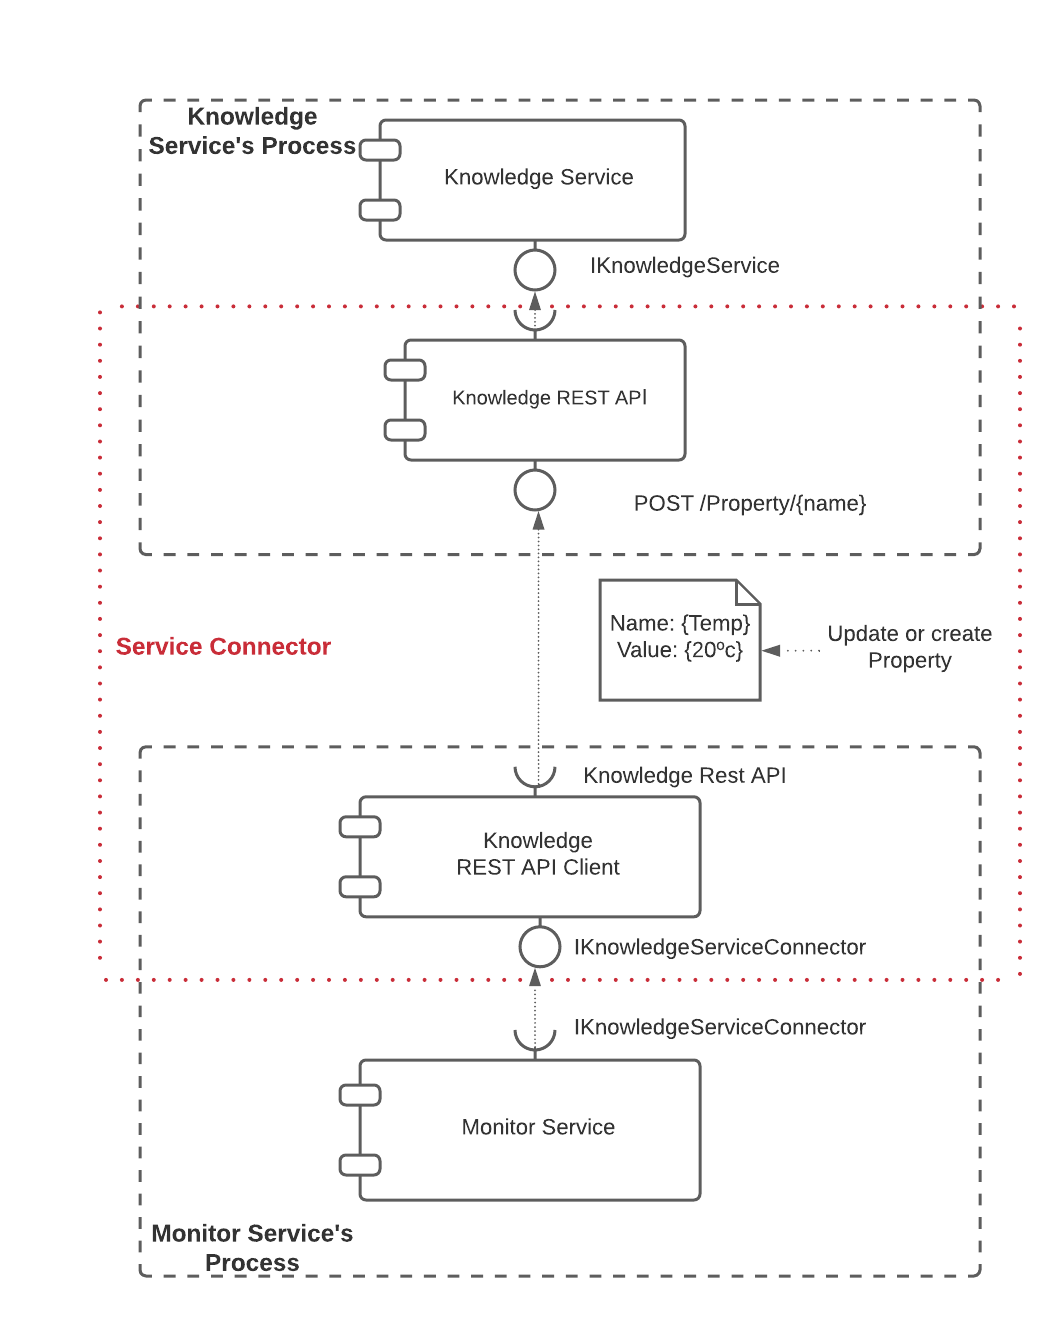
\includegraphics[scale=0.8]{03_arquitectura/images/Monitor-Knowledge-Connector}
  \caption{Diseño del conector usando implementación Cliente - Servidor}
  \label{fig:monitor-knowledge-connector-architecture}
\end{figure}

\subsection{Peticiones asíncronas}

\textbf{colas de trabajo}. \cite{royChapterMessagePatterns2017}

Las colas de trabajo consisten en un servicio enviando el publicador, que genera peticiones de trabajo y las publica en una cola. Por defecto, un consumidor, a la escucha de tareas en a cola, irá consumiendo esos mensajes.

\begin{figure}
  \centering
  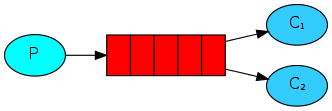
\includegraphics[scale=0.75]{03_arquitectura/images/work-queues}
  \caption[Representación de las colas de trabajo. Ejemplo de comunicación \emph{publish}-\emph{subscribe}.]{Representación de las colas de trabajo. Ejemplo de comunicación \emph{publish}-\emph{subscribe}. \footnotemark }
  \label{fig:work-queues}
\end{figure}

\footnotetext{Imagen obtenida de: \url{https://www.rabbitmq.com/tutorials/tutorial-two-dotnet.html}}

Mi idea entonces es definir dos tipos de conectores:

\begin{itemize}
  \item \textbf{Peticiones}: Utilizamos la estrategia que ya definimos en el hito anterior. Los servicios ofrecen APIs REST con una serie de operaciones. Las peticiones fluyen de microservicios más externos a los más internos, mediante llamadas HTTP.

  \begin{itemize}
    \item Por ejemplo, en el hito anterior: Probe -> Monitor -> Monitoring Service -> Knowledge

    \item Utilizamos OpenAPI para autogenerar clientes, así facilitamos la implementación de los clientes en cualquier lenguaje
  \end{itemize}

  \item \textbf{Notificaciones}: En este caso optaría por usar brokers de mensajería (o algo parecido), de forma que los microservicios de capas más internos notifican a las más externas, sin necesidad de acoplarse directamente. Cada capa estaría suscrita a los eventos de la que esté por debajo de ella. Por ejemplo: Analysis Service se suscribe a Knowledge, las Reglas de Adaptación se suscriben al Analysis Service, etc.

  \begin{itemize}
    \item Seguiría un poco la filosofía que comentamos hace un tiempo para independizar el módulo de análisis del de monitorización.

    \item Podríamos investigar la idea que has comentado, de un conector que abstraiga al cliente de esta suscripción a una cola de mensajería. A esto no le he dado muchas vueltas aun.
  \end{itemize}

\end{itemize}

